\documentclass[11pt,a4paper]{article}
\usepackage{graphicx}
\usepackage{xcolor}
\usepackage{booktabs}
\usepackage{tabularx}
\usepackage{enumitem}
\usepackage{setspace}
\usepackage{hyperref}
\usepackage{multicol}
\usepackage{caption}

% Simplify colors for Word
\definecolor{navyblue}{HTML}{003566}

\begin{document}

%  COVER PAGE - Using the high-fidelity image extracted from the PDF
\thispagestyle{empty}
\noindent
\includegraphics[width=\textwidth]{cover_page-1.png}

\newpage

\section{Background}
The Government of Madhya Pradesh, architected primarily by technical agencies such as MAP-IT and NIC, has built an impressive portfolio of digital platforms across its key departments:

\begin{itemize}
  \item \textbf{School Education:} Education Portal 3.0 is designed to manage approximately 350,000 permanent teachers.
  \item \textbf{Health:} The department operates HRMIS, NHM CHETNA, and Ayushman Sakhi.
  \item \textbf{Forest:} Uses satellite data for encroachment alerts and wildlife tourism permitting.
\end{itemize}

Institutional observation reveals a design-reality gap where day-to-day workflows still default to physical registers and informal digital tools.

\section{Rationale}
Maximizing the adoption of IT tools translates to productivity gains and structural resilience. Modernization bridges the talent drain by automating manual workarounds historically rigid in routine processing.

\section{Capacity Building Framework}
Mission Karmayogi shifts from rule-based to role-based competency. This research feeds AIGGPA’s mandate to design evidence-based modules for the iGOT platform.

\section{Theoretical Framework}
This study employs the \textbf{Unified Theory of Acceptance and Use of Technology (UTAUT)}, mapping Performance Expectancy (PE), Effort Expectancy (EE), Social Influence (SI), and Facilitating Conditions (FC).

\vspace{0.5cm}
\begin{center}
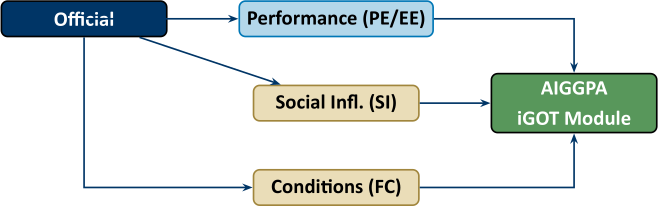
\includegraphics[width=0.8\textwidth]{figure_utaut.png}
\caption*{Figure 1. UTAUT classification flow: bureaucratic and individual barriers are coded and mapped to a targeted AIGGPA intervention.}
\end{center}

\section{Research Objectives}
\begin{itemize}
  \item Map actual tool usage across official categories.
  \item Assess document workflow and record maintenance.
  \item Capture the IT department's perspective via login statistics.
  \item Classify barriers using the UTAUT framework.
  \item Produce actionable recommendations for AIGGPA training design.
\end{itemize}

\section{Scope}
\begin{itemize}
  \item \textbf{Departments:} School Education, Health, Forest (Madhya Pradesh).
  \item \textbf{Respondents:} Class I, II, III officials and IT staff.
  \item \textbf{Duration:} April to June 2026 (10 weeks).
\end{itemize}

\section{Methodology}
This mixed-methods study uses two parallel streams:
\begin{itemize}
  \item \textbf{Stream A:} Tasks, tools, portals, and training history.
  \item \textbf{Stream B:} Platform deployment stats and IT support structure.
\end{itemize}

\subsection{Sampling Strategy}
Purposive sampling of 54 respondents analyzed as stratified case studies.

\subsection{Data Collection Instruments}
1. Semi-structured interview guide.
2. Aggregated usage statistics (IT nodal data).
3. Direct workflow observation checklist.

\subsection{Data Analysis Plan}
Manual thematic coding using ATLAS.ti, following Braun & Clarke (2006). Discrepancies between qualitative claims and numerical metrics isolate hidden blockers.

\section{Work Plan}
A 10-week schedule covering literature review, pilot testing, departmental observations (Weeks 4-8), and final report generation (Week 10).

\section{Budget Estimate}
Total Research Budget: \textbf{30,000 INR} (covering transit, software licensing, and consumables).

\section{Limitations and Ethical Considerations}
Covers access constraints, self-reporting bias, and the Hawthorne effect (mitigated via IT Ecosystem Audit). Ethical standards ensure voluntary participation and data anonymity.

\section{Expected Output}
\begin{center}
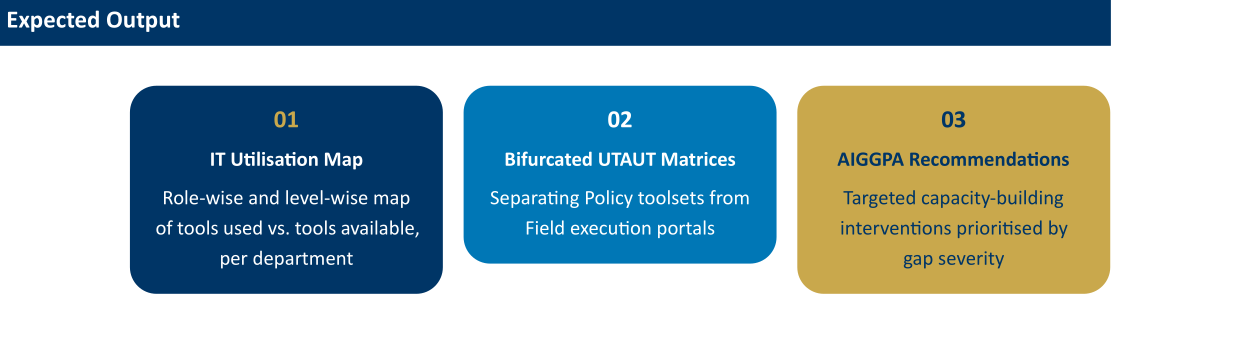
\includegraphics[width=0.9\textwidth]{expected_outputs.png}
\end{center}

\vspace{0.5cm}
\begin{center}
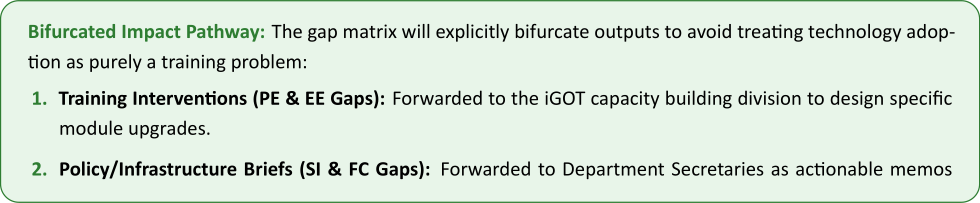
\includegraphics[width=0.9\textwidth]{impact_pathway.png}
\end{center}

\section{References}
Venkatesh, V., et al. (2003). User acceptance of information technology: Toward a unified view. \textit{MIS Quarterly}.
Heeks, R. (2003). Most IT-for-development projects fail.
Braun, V., & Clarke, V. (2006). Using thematic analysis in psychology.

\end{document}
